%version of 01-07-20

\chapter{$\oplus \oplus$ Pairing Functions: Encoding $\N^+ \times \N^+$ as $\N^+$}
\label{Appendix:building-pairing-functions}

\noindent \fbox{\begin{minipage}{0.96\textwidth}
{\bf Topic-specific references}.

\smallskip

A.L.~Rosenberg (1974): Allocating storage for extendible arrays.  {\it J.~ACM 21}, 652--670.

\smallskip

A.L.~Rosenberg (1975): Managing storage for extendible arrays.  {\it SIAM J.~Comput.~4},287--306.

\smallskip

A.L.~Rosenberg (2003): Accountable Web-computing.  {\it IEEE Trans.~Parallel and Distributed Systs.~14}, 97--106.

\smallskip

L.J.~Stockmeyer (1973): Extendible array realizations with additive traversal.  IBM Research Report RC-4578.
\end{minipage}
}

\bigskip

\noindent
This chapter extends in three directions the study of pairing functions which we began in Section~\ref{sec:pairing}.
\begin{enumerate}
\item 
We develop a ``generic" version of the construction paradigm of Section~\ref{sec:diag-pair-fn}, which develops the diagonal pairing function $\d$  of (\ref{eq:diag}) in two steps: First one decomposes $\N^+ \times \N^+$ into ``shells".  Second one linearizes the partial order of $\N^+ \times \N^+$ that the ``shells" specify.  This paradigm was motivated by the ``real-life"  challenge of devising {\em efficient} computer-storage mappings for arrays and tables that can be expanded and contracted dynamically.

\item
We describe additional specific pairing functions whose structures are specified via the ``shell"-based mechanism---and we describe inherent limitations on the ``compactness" that is achievable via the ``shell"-based paradigm.
 
\item
We exemplify a non-``shell"-based genre of pairing function which is motivated by another ``real-life" challenge: how to devise computer-storage mappings for arrays and tables whose rows can be {\em efficiently} traversed, even after an arbitrary number of dynamic expansions and contractions.  One finds one specific scenario that embodies this challenge in [Rosenberg, 2002].
\end{enumerate}
Our motivation here is twofold.  On the one hand, the mathematics needed to verify the bijectiveness of the functions we discuss provides valuable practice with some of the tools we have been developing to this point.  On the other hand, the manifold varied applications of pairing functions adds value to our excursion into the world of these functions.  The detailed survey article \cite{Rosenberg03} provides much more detail than we are able to provide here.

\bigskip

As we embark on our short guided tour, the reader should note that the diagonal pairing function of Section~\ref{sec:diag-pair-fn} and the square-shell pairing function of
Section~\ref{sec:square-pair-fn} build in essential ways on the $L$-norms of Section~\ref{sec:Ln-norms}; cf., Fig.~\ref{fig:Ln-discs}.


\section{A Shell-Based Methodology for Crafting Pairing Functions}
\label{sec:build-pair-fn}
\index{constructing pairing functions via ``shells''}
\index{pairing functions as storage mappings for arrays/tables}

The shell-oriented strategy that underlies the diagonal pairing function $\d$ can be adapted to incorporate shell-``shapes'' that are inspired by a variety of computational situations---and can be applied to computational advantage in such situations.  We describe how such adaptation can be effected, and we describe a few explicit shapes and situations.  We invite the reader to craft others.

\medskip

{\Denis Change the style for writing the algorithms -- We should guarantee the coherency all over the book!}

\noindent {\underline{\bf Procedure}} {\small\sf PF-Constructor}($\a$) \\
/*Construct a shape-inspired pairing function (PF) $\a$*/
\begin{description}
\item[Step 1.]
%
Partition the set $\N^+ \times \N^+$ into finite sets called {\it shells}.  Order the shells linearly in some way: many natural shell-partitions carry a natural order.
\end{description}
Shell $c$ of the diagonal pairing function $\d$ is the following subset of $\N^+ \times \N^+$: $\{ \langle x,y \rangle \ | \ x+y = c \}$.  The parameter $c$ orders $\d$'s shells.

\begin{description}
\item[Step 2.]
Construct a pairing function from the shells as follows.
  \begin{description}
  \item[Step 2a.]
Enumerate $\N^+ \times \N^+$ shell by shell, honoring the ordering of the shells; i.e., list the pairs in shell \#1, then shell \#2, then shell \#3, etc.
  \item[Step 2b.]
Enumerate each shell in some systematic way, e.g., ``by columns''.  In detail:

\smallskip

Enumerate the pairs $\langle x,y \rangle$ in each shell in increasing order of $y$ and, for pairs having equal $y$ values, in decreasing order of $x$.
  \end{description}
\end{description}

\begin{prop}
\label{thm:PF-construct}
Any function $\a: \N^+ \times \N^+ \leftrightarrow \N^+$ that is designed via Procedure {\small\sf PF-Constructor} is a bijection.
\end{prop}

\begin{proof}[Sketch]
Step 1 of Procedure {\small\sf PF-Constructor} constructs a partial order on $\N^+ \times \N^+$, in which: ($a$) each shell is finite; ($b$) there is a linear order on the shells.  Step 2 extends this partial order to a linear order, by honoring the inherent ordering of shells and imposing a linear order within each shell.  The function constructed via the Procedure is: {\em injective} because the disjoint shells are enumerated sequentially; {\em surjective} because the enumeration within each shell begins immediately after the enumeration within the preceding shell, with no gap.  \qed
\end{proof}

\bigskip

Having noted how to use Procedure {\small\sf PF-Constructor} to construct pairing function $\d$,  we now use the Procedure to design two other pairing functions which produce efficient atorage mappings for extendible arrays and tables..

\section{The Square-Shell Pairing Function $\s$}
\label{sec:square-pair-fn}
\index{The Square-shell pairing function $\s$}

One computational situation where pairing functions can be useful is as storage-mappings for arrays/tables that can expand and/or contract dynamically.

\medskip

In conventional programming systems, when one expands an $n \times n$ table into an $(n+1) \times (n+1)$ table, one allocates a new region of $(n+1)^2$ storage locations and copies the current table from its $n^2$-location region to the new region.  Of course, this is very wasteful: one is moving $\Omega(n^2)$ items to make room for the anticipated $2n+1$ new items.  On any given day, the practical impact of this waste depends on current technology.  But, this is a
mathematics text, not an engineering one, so we are exploring whether {\em in principle} we can avoid the waste.  The answer is ``YES''.  If we employ a pairing function $\varepsilon: \N^+ \times \N^+ \leftrightarrow \N^+$ to allocate storage for tables, then to expand a table from dimensions $n \times n$ to $(n+1) \times (n+1)$, we need move only $O(n)$ items to accommodate the {\em new} table entries; the current entries need not be moved.  For square tables, the following
{\it Square-shell} pairing function $\s$ manages the described scenario perfectly.  After describing $\s$, we comment on managing tables of other shapes.
\begin{figure}[htb]
\begin{center}
%\begin{tabular}{r|r|r|r|r|r|r|r|r}
%  1 &  4 &  9 & 16 & \fbox{25} &  36 &  49 &  64 & $\cdots$ \\
%  2 &  3 &  8 & 15 & \fbox{24} &  35 &  48 &  63 & $\cdots$ \\
%  5 &  6 &  7 & 14 & \fbox{23} &  34 &  47 &  62 & $\cdots$ \\
% 10 & 11 & 12 & 13 & \fbox{22} &  33 &  46 &  61 & $\cdots$ \\
%\fbox{17} & \fbox{18} & \fbox{19} & \fbox{20} & \fbox{21} &  32 &  45
%  &  60 & $\cdots$ \\ 
% 26 & 27 & 28 & 29 & 30 &  31 &  44 &  59 & $\cdots$ \\
% 37 & 38 & 39 & 40 & 41 &  42 &  43 &  58 & $\cdots$ \\
% 50 & 51 & 52 & 53 & 54 &  55 &  56 &  57 & $\cdots$ \\
%$\vdots$ & $\vdots$ & $\vdots$ & $\vdots$ & $\vdots$ & $\vdots$ &
%  $\vdots$ & $\vdots$ & $\ddots$
%\end{tabular}
   \includegraphics[scale=0.4]{FiguresArithmetic/PairingSquareShell}
\end{center}
\caption{{\it The square-shell pairing function $\s$.  The shell $\max(x,y) = 5$ is highlighted.}
\label{fig:pairingSquareShell}}
\end{figure}
\begin{equation}
\label{e.square}
\begin{array}{ccl}
\s(x, y) & = & m^2 + m + y-x+1 \\
           &     & \mbox{where } \ \ \  m \ \eqdef \ \max(x-1,y-1).
\end{array}
\end{equation}
One sees in Fig.~\ref{fig:pairingSquareShell} that $\s$ follows the prescription of Procedure PF-Constructor: (1) it maps integers into the ``square shells'' defined by: $m = 0, \ m = 1, ...$.  (2) it
enumerates the entries in each shell in a counterclockwise direction.  (Of course, $\s$ has a twin that enumerates the shells in a clockwise direction.)

\bigskip

\noindent \fbox{
\begin{minipage}{0.96\textwidth}
{\bf Enrichment note}.

Using somewhat more complicated instantiations of Procedure PF-Constructor, the study in [Rosenberg, 1975] adapts the square-shell pairing function $\s$ to: ($a$) accommodate, with no wastage, arrays/tables of any fixed aspect ratio $an \times bn$ ($a,b \in \N$); ($b$) accommodate, with only $O(n)$ wastage, arrays/tables whose aspect ratios come from a fixed finite set of candidates---i.e., $(a_1 n \times b_1 n)$ or $(a_2 n \times b_2 n)$ or \ldots or $(a_k n \times b_k n)$.
\end{minipage}
}

\section{$\oplus$ The Hyperbolic-Shell Pairing Function $\h$}
\label{Appendix:hyp-shell-pair-fn}
\index{The Hyperbolic-shell pairing function $\h$}

The diagonal- and square-shell pairing functions indicate that when the growth patterns of one's arrays/tables is very constrained, one can use pairing functions as storage mappings with very little wastage.  In contrast, if one employs a pairing function such as $\d$ without considering its wastage, then a storage map would show some $O(n)$-entry tables being ``spread'' over $\Omega(n^2)$ storage locations.  In the worst-case, $\d$ spreads the $n$-position $1 \times n$ array/table over $> {1 \over 2} n^2$ addresses, because: $\d(1,1) = 1$ and $\d(1,n) = {1 \over 2} (n^2 + n)$.  This degree of wastefulness can be avoided via careful analysis, coupled with the use of Procedure PF-Constructor.  The target commodity to be minimized is the {\it spread} of a PF-based storage map, which we define as follows.
\index{the spread of a pairing function}

\medskip

Note that an ordered pair of integers $\langle x,y \rangle$ appears as a position-index within an $n$-position table if, and only if, $xy \leq n$.  Therefore, we define the spread of a PF-based storage map $\m$ via the function
\begin{equation}
\label{e.compact}
{\bf S}_{\cal M}(n) \ \eqdef \ \max\{ \m(x, y) \ | \ xy \leq n \}.
\end{equation}
${\bf S}_{\cal M}(n)$ is the largest ``address'' that PF $\m$ assigns to any position of a table that has $n$ or fewer positions.

\medskip

Happily, the tools that we have developed enable us to design a pairing function that (to within constant factors) has minimum worst-case spread.  This is the {\em Hyperbolic-shell pairing function} $\h$ of (\ref{e.hyper}) and Fig.~\ref{fig:pairingHyper}.\footnote{Details appear in
[Rosenberg, 1974] and [Rosenberg, 1975].}
\begin{equation}
\label{e.hyper}
\begin{array}{lcll}
\multicolumn{4}{l}{\mbox{Let $\delta(k)$ be the number of divisors of the integer $k$.}} \\
\h(x,y) & = & {\displaystyle \sum_{k=1}^{xy-1} \delta(k) \ \ +} &
  \mbox{the position of } \ \langle x, y \rangle \ \mbox{ among 2-part} \\
        &   &  & \mbox{factorizations of the number $xy$, in} \\
        &   &  & \mbox{reverse lexicographic order}
\end{array}
\end{equation}
\begin{figure}[htb]
\begin{center}
%\begin{tabular}{r|r|r|r|r|r|r|r}
% 1 &  3 &  5 &   8 &  10 & \fbox{14} &  16  & $\cdots$ \\
% 2 &  7 & \fbox{13} &  19 &  26 &  34 &  40 & $\cdots$ \\
% 4 & \fbox{12} & 22 &  33 &  44 &  56 &  69 & $\cdots$ \\
% 6 & 18 & 32 &  48 &  64 &  81 &  99  & $\cdots$ \\
% 9 & 25 & 43 &  63 &  86 & 108 & 130  & $\cdots$ \\
%\fbox{11} & 31 & 55 &  80 & 107 & 136 & 165 & $\cdots$ \\
%15 & 39 & 68 &  98 & 129 & 164 & 200  & $\cdots$ \\
%17 & 47 & 79 & 116 & 154 & 193 & 235  & $\cdots$ \\
%$\vdots$ & $\vdots$ & $\vdots$  & $\vdots$ & $\vdots$ &
%  $\vdots$ & $\vdots$ & $\ddots$
%\end{tabular}
      \includegraphics[scale=0.4]{FiguresArithmetic/PairingHyper}
\end{center}
\caption{{\it The hyperbolic pairing function $\h$.  The shell $xy = 6$ is highlighted.}
\label{fig:pairingHyper}}
\end{figure}


\begin{prop}%[\cite{Rosenberg75}]
\label{thm:hyp-opt}
{\bf (a)}
The hyperbolic function $\h$ is a pairing function.

\smallskip

\noindent {\bf (b)}
The spread of $\h$ is given by
${\bf S}_{\cal H}(n) \ = \ O(n \log n)$.\footnote{A  detailed analysis reveals that the spread of $\cal H$ is closely related to the {\em natural} logarithm, whose base is Euler's constant $e$.}

\smallskip

\noindent {\bf (c)}
No pairing function has better compactness than $\h$ (in the worst case) by more than a constant factor.
\end{prop}

\begin{proof}
{\bf (a)} The fact that $\h$ is a pairing function follows from Proposition~\ref{thm:PF-construct}.

\smallskip

\noindent {\bf (b)}
The pairing function $\h$ maps integers along the ``hyperbolic shells'' defined by $xy = 1, \ xy =2, \ xy=3, \ldots$.  Hence, when an integer $n$ is ``placed'' into the table of values of $\h$, the number of occupied slots is within $n$ of
\[ \sum_{i=1}^{n-1} \ |\{ \langle x,y \rangle \ | \ xy < i \}|  \]
Elementary calculations show that this sum is $O(n \log n)$.

\smallskip

\noindent {\bf (c)}
The optimality of $\h$ in compactness (up to constant factors) is seen via the following argument.  The set of tables that have $n$ or fewer positions are those of aspect ratios $a_i \times b_i$, where $a_i b_i \leq n$.  As one sees from Fig.~\ref{f.hyp} (generalized to arbitrary $n$), the union of the positions of all these arrays is the set of integer lattice points under the hyperbola $xy = n$.  It is well-known---cf.~\cite{NivenZ80}---that this set of points has cardinality $\Theta(n \log n)$.  Since every table contains position $\langle 1,1 \rangle$, it follows that, for every $n$, some table containing $n$ or fewer positions is spread over $\Omega(n \log n)$ ``addresses.''  \qed
\end{proof}
\begin{figure}[htb]
\begin{center}
       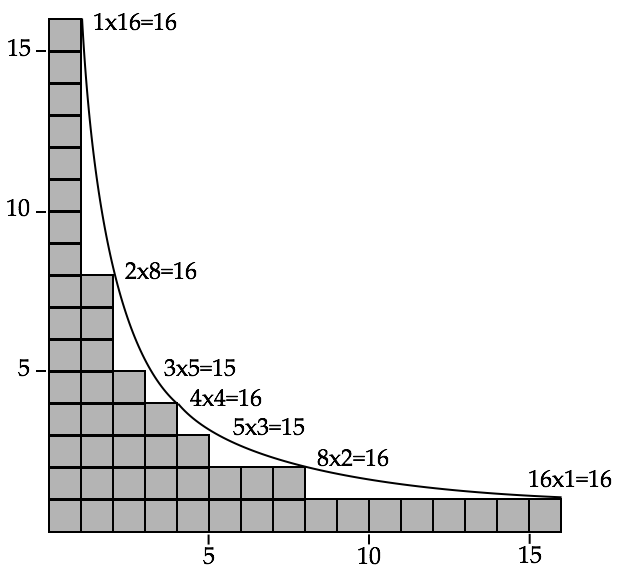
\includegraphics[scale=0.4]{FiguresArithmetic/PairingHyp}
\caption{The aggregate set of positions of tables having $16$ or fewer position.  To help the reader understand the figure, we include the curve $f(x,y) = xy$ which provides an upper envelope for the set.  A careful look at this curve will reveal that it touches the set of positions at the points $\langle x,y \rangle \in \{ \langle 1,16 \rangle, \ \langle 2,8 \rangle, \ \langle 4,4 \rangle, \ \langle 8,2 \rangle, \ \langle 16,1 \rangle \}$, but it does {\em not} touch the set at the points $\langle x,y \rangle \in \{ \langle 3,5 \rangle, \ \langle 5,3 \rangle \}$. 
\label{f.hyp}}
\end{center}
\end{figure}

\section{A Pairing Function Built from Disjoint Arithmetic Progressions}

As we noted earlier, the notion of pairing function has applications to a broad range of computational situations.  For some of these---cf., \cite{Rosenberg03}---it is convenient to have each ``row'' of the pairing function map onto an arithmetic progression.  This can be achieved in many ways, as explained in \cite{Rosenberg03}.  For this section, we satisfy ourselves with presenting a single such {\em additive} pairing function, let us call it $\a(x,y)$.  The reader can find a comprehensive study of such pairing functions in [Stockmeyer, 1973].

\medskip

\noindent
For all $\langle x,y \rangle \in \N^+ \times \N^+$

$\a(x,y) \ \eqdef \ 2^{x-1} \cdot (2y -1)$

\noindent
We leave to the reader the exercise of verifying function $\a$'s bijectiveness.  As an aid, we provide the following prefix of $\a$'s mapping of $\N^+ \times \N^+$.
\begin{center}
\begin{tabular}{r|r|r|r|r|r|r}                                                               
 1 &  3 &   5 &   7 &   9 &  11 & $\cdots$ \\                                      
 2 &  6 &  10 &  14 &  18 &  22 & $\cdots$ \\                                      
 4 & 12 &  20 &  28 &  36 &  44 & $\cdots$ \\                                      
 8 & 24 &  40 &  56 &  72 &  88 & $\cdots$ \\                                            
16 & 48 &  80 & 112 & 144 & 176 & $\cdots$ \\
32 & 96 & 110 & 224 & 288 & 352 & $\cdots$ \\                                      
$\vdots$ & $\vdots$ & $\vdots$  & $\vdots$ & $\vdots$ & $\vdots$ & $\ddots$
\end{tabular} 
\end{center}
